% Manuscript for IEEE Transactions on Learning Technologies (TLT).
% Venue chosen 2026-11-17 (supervisor: IEEE first; owner: TLT). See docs/research-outline.md.
% TLT rules (TLT author resources, effective 2025-01-01): regular paper <= 14 pages in the
% final IEEE double-column format (extra pages cost a fee); short paper <= 8. Submit via IEEE Author Portal.
% TODO before submission: confirm the class options with https://template-selector.ieee.org/
% (journal vs compsoc), and whether review is single- or double-blind.
% Build (from manuscript/): mkdir -p build && tectonic -X compile main.tex --outdir build  -> build/main.pdf (git-ignored)
% Every number must come from docs/results/*.md (which cite results/); never type a number from memory.
\documentclass[journal]{IEEEtran}
\usepackage{graphicx}
\usepackage{booktabs}
\usepackage{amsmath}
\usepackage{url}
\usepackage{iftex}
\ifXeTeX\usepackage{fontspec}\setmainfont{texgyretermes}[Extension=.otf,UprightFont=*-regular,BoldFont=*-bold,ItalicFont=*-italic,BoldItalicFont=*-bolditalic]\fi % local tectonic build only; Overleaf/pdflatex uses IEEEtran's Times
\graphicspath{{../docs/results/figures/}}

\begin{document}

% Working title: say the finding, not only the topic.
\title{A Fine-Tuned Small Model Outgrades a Larger One on the Edge:\\
Accuracy, Latency and Energy of Short-Answer Grading on a Jetson Orin Nano}

\author{Dhista~Ardiansyah% TODO: co-authors, affiliations, IEEE membership
\thanks{TODO: affiliation, funding (TEEP), corresponding author.}}

\markboth{IEEE Transactions on Learning Technologies}{Ardiansyah \MakeLowercase{\textit{et al.}}: Fine-Tuned Small Graders on the Edge}

\maketitle

\begin{abstract}
% Draft. Numbers: docs/results/jetson-graders.md (three graders, 612 MHz, 2026-11-14 to 11-16).
Grading short answers takes teachers much time, and cloud language models raise cost, privacy and connectivity concerns for schools.
We ask whether a small language model, fine-tuned and run on a low-power edge board, can replace a larger untouched one.
On SciEntsBank (3-way labels), we compare Gemma~4 E2B untouched, E2B with a QLoRA adapter, and E4B untouched, all served by llama.cpp on a Jetson Orin Nano.
On unseen questions and unseen domains, the fine-tuned E2B scores 76.7\% and 74.8\%, beating untouched E4B by 9.4 and 4.7 points (paired McNemar, Holm $p<10^{-6}$),
while using about 22\% less energy (5.3--5.4~J against 6.8--6.9~J per answer) and answering about 20\% faster (0.57~s against 0.70~s).
Fine-tuning costs 9--11~J per extra correct answer, against 31--41~J for moving to the larger model and 830--1{,}340~J for turning thinking on.
% TODO: thinking-on adapter runs (2026-11-17), Beetle/SAF transfer, one closing sentence for teachers.
\end{abstract}

\begin{IEEEkeywords}
% TODO: pick from the IEEE taxonomy.
Automatic short answer grading, small language models, fine-tuning, edge computing, energy efficiency.
\end{IEEEkeywords}

\section{Introduction}
% Sources: docs/research-outline.md ("Why", RQ4, RQ8); research_notes/Recent short answer grading benchmarks/usage_in_papers.md (gap).
\IEEEPARstart{S}{hort-answer} questions ask students to explain an idea in their own words, which shows understanding better than a choice among options, but every answer has to be read and graded.
That work falls on teachers, and it grows with every class and every test.
Automatic short-answer grading has been studied for over a decade~\cite{dzikovska2013semeval}, and large language models now match or beat the best earlier systems on its benchmarks~\cite{wang2024rag,funayama2025crossprompt}.

The strongest of these results, however, come from large models reached through a cloud service.
For a school, that means a fee for every graded answer, student work leaving school hardware, a dependence on a network connection, and a model that can change without notice; earlier work raises the same concerns about transparency, security, privacy and hardware cost~\cite{ormerod2024gpupoor,saur2026grading}.
A small model running on a board inside the school avoids all four.
Small open models, fine-tuned and often with low-rank adapters, are already common in grading research~\cite{ormerod2024gpupoor,aggarwal2024engsaf,walsh2025finetuning,funayama2025crossprompt}, yet they are evaluated for accuracy, mostly on server GPUs.
The closest on-device study we found times models of up to about one billion parameters on a laptop CPU~\cite{saur2026grading}; studies of language models on edge accelerators measure power and latency, but not on grading~\cite{arya2025edgepower}.
To our knowledge, no grading study has reported energy per graded answer, or run on an edge board.

That missing cost matters for the choice a school actually faces.
A school device has a fixed power budget, and a teacher waits for the grades, so an accuracy gain counts only next to the time and energy it adds.
The obvious way to grade better is a larger model; the alternative is to adapt a smaller one to the task.
We ask: \textit{can a fine-tuned small grader replace a larger untouched one on an edge device, and what does each accuracy gain cost there?}

We answer with three graders built on Gemma~4: E2B untouched, E2B fine-tuned (``tweaked''), and E4B untouched, the next size up.
All three grade the SciEntsBank benchmark on an NVIDIA Jetson Orin Nano, and we measure accuracy on questions and domains never seen in training, together with latency and energy per answer on the board.
We also measure the other ways one might raise a small grader's accuracy (more training seeds and their average, finer labels, written reasons, graded examples in the prompt, course material retrieved into the prompt, and thinking before answering) on the same board.
Our contributions are:
\begin{itemize}
\item A controlled comparison on unseen questions and unseen domains, showing that fine-tuned E2B beats untouched E4B by 9.4 and 4.7 points while using about 22\% less energy and answering about 20\% faster per answer.
\item Measured device cost for every grader, and \textit{energy per extra correct answer} as a single price for an accuracy gain: 9--11~J for fine-tuning, against 31--41~J for the larger model and 830--1{,}340~J for thinking on.
\item Evidence that the extras do not pay on the device: no other way of tweaking E2B beat a plain adapter, retrieved course material did not help grading, and each extra added energy per answer, from 4\% for the averaged adapter to over seven times for written reasons.
\end{itemize}
% TODO: last bullet or sentence on releasing code, run summaries and adapters, if the owner agrees.

Section~II reviews related work, Section~III describes the data, graders and measurement, Section~IV gives the results, and Section~V discusses what they mean for schools and where they stop.

\section{Related Work}
\subsection{Short-Answer Grading and SciEntsBank}
% SemEval-2013 Task 7 \cite{dzikovska2013semeval}; splits ua/uq/ud; accuracy + macro-F1, not QWK (categorical labels). research_notes/Recent short answer grading benchmarks/.
\subsection{Language Models as Graders}
% Prompting, graded examples, RAG, fine-tuning (LoRA/QLoRA \cite{hu2022lora,dettmers2023qlora}). research_notes/2026-11-13-llm-finetuning-on-scientsbank.md.
\subsection{Small Models on Edge Devices}
% On-device latency/energy studies; why a Jetson-class board fits a school budget.

\section{Method}
% Sources: docs/research-outline.md (setup), docs/results/finetuning.md, examples.md, jetson-graders.md,
% results/finetune/finetune-e2b-20261027-111124.json, src/edge_grader/grader.py (prompt).

\subsection{Dataset and Splits}
We use SciEntsBank, the science part of the SemEval-2013 Task~7 student response analysis challenge~\cite{dzikovska2013semeval}.
% TODO verify against the SemEval paper: grades 3--6, ASK assessments.
Each item gives a question, a reference answer and a student answer, with an expert label.
We use the 3-way labels (\textit{correct}, \textit{contradictory}, \textit{incorrect}), which are categories rather than an ordered scale, so we report accuracy and macro-F1, the metrics of the shared task, rather than quadratic weighted kappa.
The training split has 4{,}969 answers.
The test data come in three splits: unseen answers (test\_ua, 540 answers), unseen questions (test\_uq, 733 answers to 15 questions) and unseen domains (test\_ud, 4{,}562 answers to 46 questions).
Because test\_ua's questions also appear in training, a fine-tuned grader has seen them; for every fine-tuned version we therefore treat test\_uq and test\_ud as the headline splits and report test\_ua only as context.

\subsection{Models and Serving}
The graders are Gemma~4 E2B and E4B, instruction-tuned and quantization-aware-trained, served as 4-bit GGUF files (\texttt{UD-Q4\_K\_XL}) by \texttt{llama-server} from llama.cpp.
% TODO cite Gemma 4 model card and llama.cpp.
Every run uses the same settings: an 8{,}192-token context, all layers on the GPU, thinking off unless stated, temperature~0 (greedy decoding), and one run per split.
The prompt (Fig.~\ref{fig:prompt}) gives the question, the reference answer, the student answer and a one-line description of each label, and asks for the label only.
The first label word in the reply is taken as the grade; a reply that names no label counts as wrong.

\begin{figure}[t]
\centering
\begin{minipage}{0.95\columnwidth}
\scriptsize
\begin{verbatim}
You are grading a student's answer to a science question.

Question: {question}
Reference answer: {reference_answer}
Student answer: {student_answer}

Choose exactly one label:
- correct: a complete and correct answer
- contradictory: contradicts the reference answer
- incorrect: partially correct, incomplete, irrelevant,
  or off-topic

Reply with the label only.
\end{verbatim}
\end{minipage}
\caption{Grading prompt, the same for every grader. Variants add course passages (RAG) or graded examples before the question.}
\label{fig:prompt}
\end{figure}

\subsection{Fine-Tuning}
We fine-tune each model with QLoRA~\cite{dettmers2023qlora}: low-rank adapters~\cite{hu2022lora} of rank~16 ($\alpha=32$, dropout 0.05) on every attention and feed-forward projection of the language model, over a frozen base loaded in 4-bit NF4 with double quantization.
Training uses a learning rate of $2\times10^{-4}$ with a cosine schedule and 3\% warm-up, an effective batch of 16 (1 answer $\times$ 16 accumulation steps) and at most three epochs, on one NVIDIA T4 GPU.
The training target is the label alone.
We hold out 14 training questions (499 answers) and keep the epoch that grades them best (epoch~2 for E2B, at 78.8\%).
The adapter is converted to GGUF and loaded beside the unchanged quantized model with llama.cpp's \texttt{--lora} option, without merging.
We call this adapter ``E2B tweaked''.

\subsection{Other Ways to Tweak E2B}
To check that a plain adapter is E2B's best fine-tuned version, we also tried the methods we had first tested on E4B:
\begin{itemize}
\item \textit{Seeds and a model soup:} five adapters with seeds 0--4, and their uniform average~\cite{wortsman2022soups}.
\item \textit{5-way labels:} the adapter trained to reply with SciEntsBank's five labels, mapped to 3-way for scoring.
\item \textit{Reasons with the label:} adapters trained to give a short reason after the label (label-first) or before it (reason-first). The reasons were written by Qwen3-14B given the gold label; 4{,}819 of 4{,}969 were kept after an automatic check, and the first author judged 27 of 30 sampled reasons faithful.
\item \textit{Graded examples in the prompt:} four graded training answers, chosen either as nearest neighbours of the item by \texttt{bge-small-en-v1.5} embeddings or at random, placed before the question; tried on the untouched model and on the adapter.
\end{itemize}
The seeds, soup, 5-way and example runs were graded on an NVIDIA DGX Spark first; their labels on the Jetson agree with the Spark's on 97.4--99.9\% of answers per run.

\subsection{Device Measurement}
All three graders and every E2B version were graded on one NVIDIA Jetson Orin Nano, an embedded board of the kind a school could keep on site.
The GPU clock was 612~MHz and the memory clock 2{,}133~MHz on every run, and the untouched models were re-run in the same queue as the tweaked ones, so every comparison is within one clock state and one llama.cpp build.
Power is the board's DC draw summed over its INA3221 rails, sampled at 1~Hz; it is not wall power.
Energy is integrated over the grading window, from the first request to the last, and divided by the number of answers.
We also report the median latency per answer and the decode speed (tokens/s) from \texttt{llama-server}'s own timings.
To compare a gain with its price we use the \textit{energy per extra correct answer}, the extra joules per answer divided by the gain in accuracy.

\subsection{Statistics}
Graders are compared on the same answers with a paired McNemar test~\cite{mcnemar1947}, and the $p$-values are corrected with Holm's method~\cite{holm1979} over a family of eight comparisons.
The family was fixed after the runs; since the largest corrected $p$ in it is 0.0003, a different family would not change the conclusions.
For each accuracy we give a 95\% interval from 2{,}000 bootstrap resamples of whole questions, since answers to one question are not independent.

\section{Results}

\subsection{Three Graders}
Table~\ref{tab:three} gives accuracy and cost for the three graders, and Table~\ref{tab:tests} the paired tests.
Fine-tuning lifts E2B by 16.9 points on unseen questions and 14.6 on unseen domains, which takes it past untouched E4B by 9.4 and 4.7 points; both differences hold after correction ($p<10^{-6}$), on the 3-way labels and on the 2-way (correct against not correct) labels.
The bootstrap intervals overlap on test\_uq, which has only 15 questions; the paired tests, which compare the same answers, are the stronger evidence.
Untouched E4B's lead over untouched E2B appears only on the 3-way labels: on 2-way the two differ by $-3.1$ and $+1.0$ points and not significantly different, so E4B's advantage is in telling \textit{contradictory} from \textit{incorrect}.
E4B with its own adapter is the most accurate grader we measured (80.0\% and 76.7\%).

\begin{table*}[t]
\centering
\caption{Accuracy and Cost of the Graders on the Jetson Orin Nano (3-Way Labels)}
\label{tab:three}
\begin{tabular}{@{}lccccc@{}}
\toprule
Grader & test\_uq acc.\ (95\% interval) & test\_ud acc.\ (95\% interval) & Macro-F1 uq / ud & Median latency (s) & Energy (J/answer) \\
\midrule
E2B untouched & 59.8 (50.1--69.2) & 60.2 (54.9--65.0) & 0.548 / 0.570 & 0.40--0.41 & 3.7--3.8 \\
\textbf{E2B tweaked} & \textbf{76.7} (68.3--84.9) & \textbf{74.8} (69.5--79.4) & 0.755 / 0.746 & 0.56--0.58 & 5.3--5.4 \\
E4B untouched & 67.3 (58.5--77.3) & 70.1 (64.9--74.3) & 0.650 / 0.701 & 0.70--0.71 & 6.8--6.9 \\
\midrule
\textit{E4B tweaked (reference)} & 80.0 (73.0--86.3) & 76.7 (72.0--81.2) & 0.786 / 0.775 & 0.93--0.97 & 9.3--9.5 \\
\bottomrule
\end{tabular}
\\[2pt]
\footnotesize Ranges in the last two columns span the two splits.
\end{table*}

\begin{table}[t]
\centering
\caption{Paired Comparisons (Accuracy Difference in Points; Holm-Corrected McNemar)}
\label{tab:tests}
\footnotesize
\setlength{\tabcolsep}{3pt}
\begin{tabular}{@{}lcc@{}}
\toprule
Comparison & test\_uq & test\_ud \\
\midrule
E2B tweaked vs E2B untouched & +16.9 (163/39) & +14.6 (912/248) \\
E2B tweaked vs E4B untouched & +9.4 (127/58) & +4.7 (584/369) \\
E4B untouched vs E2B untouched & +7.5 (140/85) & +9.8 (820/371) \\
E4B tweaked vs E4B untouched & +12.7 (138/45) & +6.6 (663/361) \\
\bottomrule
\end{tabular}
\\[2pt]
\raggedright In brackets: answers only the first grader got right / only the second. All eight tests: corrected $p\le0.0003$.
\end{table}

\subsection{Cost on the Device}
E2B tweaked is cheaper to run than E4B untouched: about 20\% faster per answer (0.57~s against 0.70~s) and about 22\% lower in energy (5.3--5.4~J against 6.8--6.9~J).
The adapter itself is not free: at the same prompt and the same two-token reply, it costs E2B 42\% more energy than the untouched model.
llama.cpp applies an unmerged adapter beside the weights on every token, so decoding drops from 40.7 to 26.9 tokens/s and prefill slows from 1.4 to 2.1~ms per prompt token.
Even so, fine-tuning is the cheapest accuracy gain we measured: 9--11~J per extra correct answer, against 31--41~J for moving from E2B to E4B, and 126--210~J for moving from E2B tweaked to E4B tweaked.
Fig.~\ref{fig:acc-energy} places every grader on accuracy against energy: E2B tweaked sits above and to the left of E4B untouched on both splits, and the E2B versions that edge above it cost the same or more.

\begin{figure*}[t]
\centering
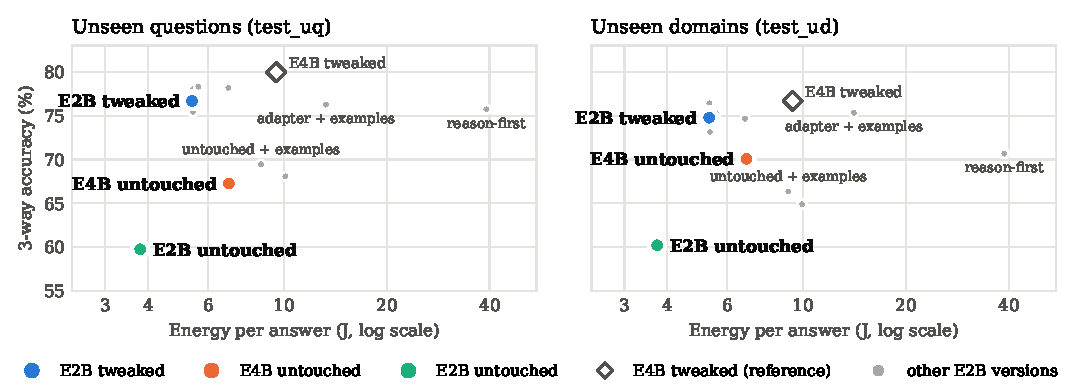
\includegraphics[width=\textwidth]{jetson-three-graders.pdf}
\caption{Accuracy against energy per answer on the Jetson Orin Nano (612~MHz GPU clock). Up and to the left is better. Grey points are the other E2B versions of Table~\ref{tab:variants}: the unlabelled cluster beside E2B tweaked holds the five seeds, their soup, the label-first adapter and, at 6.8--6.9~J, the 5-way adapter; ``untouched + examples'' marks the nearest and the random graded examples. Drawn by \texttt{scripts/paper\_figures.py} from the run comparison file.}
\label{fig:acc-energy}
\end{figure*}

\subsection{Other Tweaks Add Cost, Not Accuracy}
Table~\ref{tab:variants} lists every fine-tuned E2B version.
All plain adapters (the five seeds, their soup and the one we use) land within one band, 75--78\% on test\_uq and 74--76\% on test\_ud, at 5.3--5.6~J; the seeds alone span 2--3 points, so differences inside the band are training noise.
Neither the soup nor the 5-way adapter was significantly better than a single seed.
The extras only add cost: 5-way labels add a third reply token and 28\% energy; graded examples on the adapter raise the prompt from about 160 to 550--630 tokens and cost 2.5--2.7$\times$ its energy; a written reason before the label takes 63--64 tokens per answer and 7.3$\times$ the energy, at 4.3~s per answer, with no gain in accuracy.
Without training, graded examples do lift untouched E2B (to 69.4\% and 66.3\%), but at 2.3--2.4$\times$ its energy, and still below the adapter.

\begin{table}[t]
\centering
\caption{Every Fine-Tuned E2B Version on the Jetson}
\label{tab:variants}
\footnotesize
\setlength{\tabcolsep}{3pt}
\begin{tabular}{@{}lccc@{}}
\toprule
E2B version & test\_uq & test\_ud & J/answer \\
\midrule
untouched & 59.8 & 60.2 & 3.7--3.8 \\
adapter (E2B tweaked) & 76.7 & 74.8 & 5.3--5.4 \\
seeds 0--4 (range) & 75.4--78.0 & 74.4--76.4 & 5.3--5.4 \\
soup of seeds 0--4 & 78.3 & 75.3 & 5.5--5.6 \\
5-way labels & 78.2 & 74.7 & 6.8--6.9 \\
label-first reason & 76.1 & 73.1 & 5.3--5.4 \\
reason-first & 75.7 & 70.7 & 38.8--39.2 \\
adapter + nearest examples & 76.3 & 75.3 & 13.3--14.1 \\
\midrule
\textit{untouched + nearest examples} & 69.4 & 66.3 & 8.6--9.1 \\
\textit{untouched + random examples} & 68.1 & 64.9 & 9.9--10.1 \\
\bottomrule
\end{tabular}
\end{table}

\subsection{Is the Gain Memorized Questions?}
SciEntsBank's unseen-question and unseen-domain splits share no questions with training, but they come from the same assessments.
As a check that does not depend on SciEntsBank at all, we trained the same E2B adapter on two other grading sets, Beetle and SAF, and graded SciEntsBank with it.
% TODO cite Beetle (also SemEval-2013 Task 7) and SAF.
It scores 76.7\% on test\_uq, the same as the SciEntsBank adapter, but 68.2\% on test\_ud, so the gain transfers in part: on unseen domains, part of it is specific to SciEntsBank.

\subsection{Course Material (RAG) Does Not Help Grading}
Adding the three most relevant textbook passages to the prompt (retrieved with \texttt{bge-small-en-v1.5} from open school science textbooks and Wikipedia) did not improve grading.
E2B lost 2.9 points on test\_uq and 5.1 on test\_ud (the latter significant, $p<0.001$); E4B changed by $+2.9$ and $+0.3$ points, neither significant.
% Kaggle T4 runs, same build and prompt (docs/results/rag.md); Jetson cost of RAG in docs/results/variations.md.
The passages raised recall on \textit{correct} answers but lowered it on \textit{incorrect} ones: they made the model more lenient rather than more accurate.

\subsection{Thinking On}
With thinking on (a 320-token thinking budget), untouched E2B reaches 75.7\% on test\_uq and 70.1\% on test\_ud, close to the adapter on unseen questions though not on unseen domains, but at 13.7~s and 136.7--136.9~J per answer: 830--1{,}340~J per extra correct answer, roughly a hundred times the adapter's price.
% TODO: thinking on with each adapter (Jetson runs of 2026-11-16/17, results/board/*think*).

\subsection{Against Published Results}
% Single runs with one seed and one prompt; the published systems differ in prompt, training and evaluation code.
On the same splits and metric, the best published 3-way accuracies we found are 76.9\% (test\_uq) and 73.4\% (test\_ud), from Claude~3.5 Sonnet with retrieval~\cite{wang2024rag}.
E2B tweaked, a 4-bit model on a low-power board, is on a par with them (76.7\% and 74.8\%), and well above the best systems of the original shared task (65.3\% and 64.0\%).

\section{Discussion}
% What this means for a school: grades per hour, Wh per class set; when E4B + adapter is worth 1.8x energy.
\subsection{Limitations}
% SciEntsBank leakage worry (test_ua); English only; one board and one clock state; no merged adapter tested; cloud comparison (RQ5) not run.

\section{Conclusion}
% TODO

\nocite{*} % shortcut: lists every refs.bib entry while the cites sit in comments; drop once the text cites them
\bibliographystyle{IEEEtran}
\bibliography{refs}

\end{document}
